\documentclass[11pt, oneside]{article}   	% use "amsart" instead of "article" for AMSLaTeX format
\usepackage{geometry}                		% See geometry.pdf to learn the layout options. There are lots.
\geometry{letterpaper}                   		% ... or a4paper or a5paper or ... 
%\geometry{landscape}                		% Activate for for rotated page geometry
%\usepackage[parfill]{parskip}    		% Activate to begin paragraphs with an empty line rather than an indent
\usepackage{graphicx}				% Use pdf, png, jpg, or eps� with pdflatex; use eps in DVI mode
								% TeX will automatically convert eps --> pdf in pdflatex		
\usepackage{amssymb}
\usepackage{amsmath}
\usepackage{parskip}
\usepackage{color}

\title{Schey Ch. 2, part 1}
%\author{The Author}
%\section{}
% \subsection*{R code}
\date{}							% Activate to display a given date or no date

\graphicspath{{/Users/telliott_admin/Dropbox/Tex/png/}}

% \begin{center} 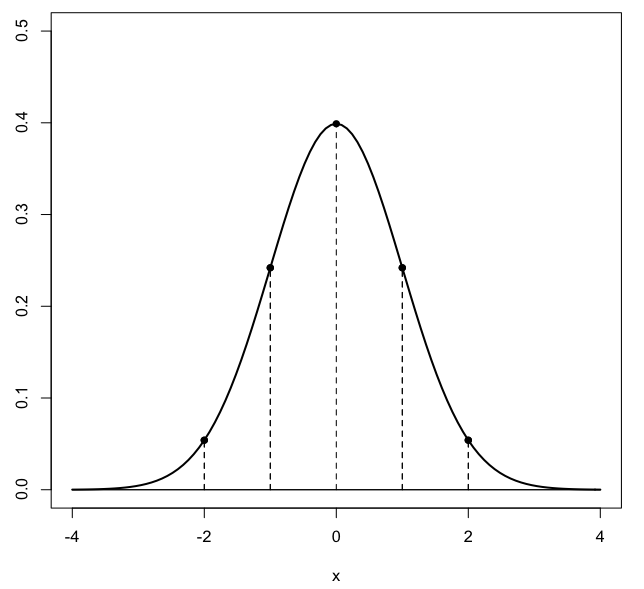
\includegraphics [scale=0.4] {gauss3.png} \end{center}
% \begin{bmatrix} a  &  b \\ c  &  d \end{bmatrix}
% \bigg |_

\begin{document}
\maketitle
\large
%\noindent

We are going to follow along with Schey's book, taking notes.  He tries to motivate the reader for what's ahead with Gauss's Law

\[ \iint_S \mathbf{E} \cdot \hat{\mathbf{n}} \ dS = \frac{q}{\mathbf{\epsilon_o}} \]

We find the value of the dot product of the electric field with the unit normal vector to the surface, and integrate these over the entire surface.  The result is proportional to the total charge contained inside the surface, $q$.  We need to find expressions for the normal vector and the surface element $dS$.  It will turn out that the combination is simpler than either one alone, because of a cancellation:

\[ \hat{\mathbf{n}} \ dS = < -f_x,-f_y,1>  \ dx \ dy \]

\subsection*{normal vector}

The first topic is the normal vector to a surface at a point $P$.  If we have two vectors in a plane, $\mathbf{u}$ and $\mathbf{v}$, we know that their cross-product $\mathbf{u} \times \mathbf{v}$ produces a vector perpendicular to both $\mathbf{u}$ and $\mathbf{v}$.  If we have a curving surface, taking any two (different) vectors which are tangent to the surface at $P$, will give an identical result.  To normalize the resulting vector, producing a unit vector, we must divide by its magnitude.

\[  \hat{\mathbf{n}} = \frac{\mathbf{u} \times \mathbf{v}}{| \mathbf{u} \times \mathbf{v} |} \]

A simple surface might be specified as $z = f(x,y)$.  For convenience, Schey specifies a plane parallel to the $xz$-axis at some point $P$, passing through the surface $f(x,y)$.  The intersection of the surface and this plane traces out a curve, and the tangent vector at any point can be taken to have some (arbitrary) length $u_x$ in the $x$-direction.  Its $z$-component is equal to the slope of the surface in the $x$-direction at that point, times that length.  The change in $z$ is $\partial f / \partial x \  u_x$ and our vector will be

\[ <\frac{\partial f}{\partial x}, 0,  \frac{\partial f}{\partial x} \ u_x> \]

\begin{center} 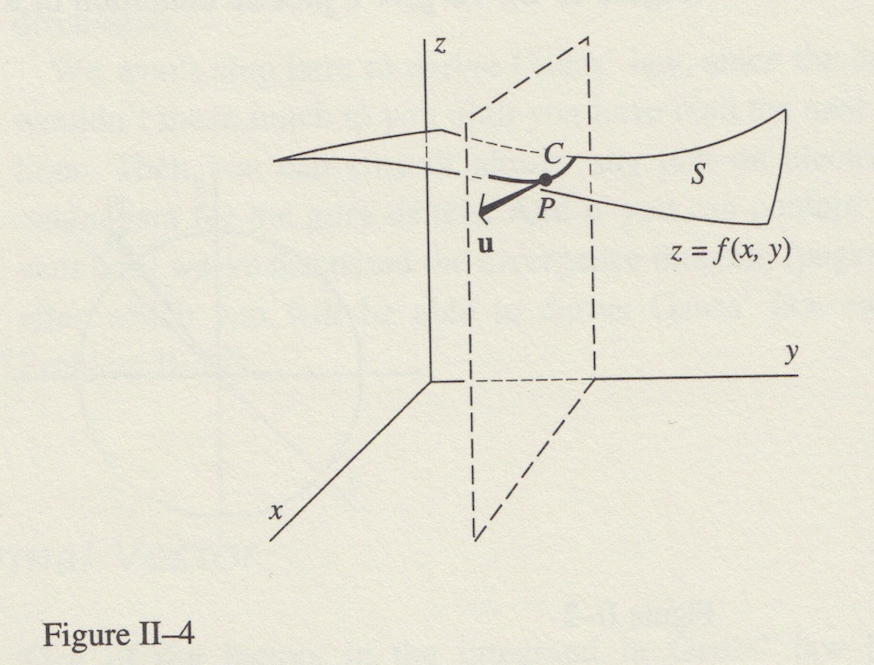
\includegraphics [scale=0.3] {intersect.png} \end{center}

However, (following Auroux), I like to use an alternative notation for the partial derivative

\[ \frac{\partial f}{\partial x}  = f_x \]
It is a lot simpler, as long as you don't get confused about which $f$ you are talking about (like the $x$ component of $\mathbf{F}$, which is different).
  
Also, we should recognize that the vectors we use don't have to be parallel to the $xz$-plane.  For example, they could be in terms of $u,v$ parametrizing the surface.  In the general case we have

\[ \mathbf{u} = \ < \ \Delta u, 0, f_u \ \Delta u \ > \]

This is the linear approximation to $f(u + \Delta u)$

Similarly for a plane containing the vector $v$

\[ \mathbf{v} = \ < 0, \Delta v,  f_y \ \Delta v > \]

So
\[ \mathbf{u} \times \mathbf{v} =  < \Delta u, 0,  f_x \ \Delta u \ > \times \ < 0, \Delta v,  f_y \ \Delta v > \]
At this point let's factor out $\Delta u \ \Delta v$
\[ =  \Delta u \ \Delta v \ < 1, 0,  f_x  > \ \times \ < 0, 1,  f_y  > \]
The cross-product is
\[ 
\begin{vmatrix}
\hat{\mathbf{i}} & \hat{\mathbf{j}} & \hat{\mathbf{k}}  \\
1 & 0 & f_x \\
0& 1 & f_y
\end{vmatrix}
\]
\[ \mathbf{n} =  \Delta u \ \Delta v \ <-f_x,-f_y,1> \]
To get the unit vector, we need to divide by the magnitude of $\mathbf{n}$.  The factor of $\Delta u \ \Delta v$ will be in the denominator as well, and cancel, leaving

\[  \hat{\mathbf{n}}  = \frac{1}{\sqrt{f_x^2  + f_y^2 + 1}} \ < \ -f_x, - f_y , 1  \ > \]

\noindent\rule{15cm}{0.4pt}

\subsection*{examples}

Here are two examples.  First, the $xy$-plane.  That is

\[ z = f(x,y) = 0 \]

Of course, $f_x = 0$, and so does $f_y$. So the normalizing constant for $\mathbf{n}$ above is just equal to $1$.  We are left with 

\[  \hat{\mathbf{n}} =  \ < \ -f_x, - f_y  , 1  \ > =  \ < \ 0, 0, 1 \ >   \] 

Second, the sphere centered on the origin of radius $r$

\[ x^2 + y^2 + z^2 = r^2 \]
\[ z = \sqrt{r^2 - x^2 -y^2} \]
\[ f_x = \frac{1}{2} \ \frac{-2x}{\sqrt{r^2 - x^2 -y^2}} = -\frac{x}{z} \]
\[ f_y = -\frac{y}{z} \]

The normal vector is
\[ = \frac {1}{\sqrt{\frac{x^2}{z^2}  +\frac{y^2}{z^2} + 1}}  \ < \ \frac{x}{z}, \frac{y}{z}, 1 \ > \]
multiply top and bottom by $z$
\[ = \frac {1}{\sqrt{x^2  + y^2 + z^2}}  \ < \ x, y, z \ > \]
\[ =  \frac{1}{r}  \ < \ x, y, z \ > \]
The radial vector.  And its length is equal to $r$ since

\[ | \frac{1}{r} \ < \ x, y, z \ >  | = \frac{1}{r} \ \sqrt{x^2 + y^2 + z^2} = 1 \]

\noindent\rule{15cm}{0.4pt}

\subsection*{surface integrals}

The next step is to think about surface integrals.  In the original example

\[ \iint_S \mathbf{E} \cdot \hat{\mathbf{n}} \ dS = \frac{q}{\mathbf{\epsilon_o}} \]

both $ \mathbf{E}$ and $\hat{\mathbf{n}}$ are functions of $x,y,z$.  We imagine dividing up the surface into lots of planar little area elements dS, each of which is tangent to the surface at some point within dS, and having a normal vector at the same point.  We compute the dot product at the point, and sum over all the area elements.

In order to actually do this integral, we will need to reduce the number of variables from $3$ to $2$, from $x,y,z$ to $x,y$, for example, by using the fact that $z = f(x,y)$.

We can do this type of integral with scalar functions, such as

\[ \iint_S G(x,y,z)  \ dS \]

which saves us from thinking about the dot product for a minute.

Now, we need to think carefully about the area of the surface elements.  Suppose we use rectangles arranged on the surface, which are always oriented with one pair of (opposing) sides parallel to the $xy$-plane (not necessarily parallel to the $x$ and $y$-axes.  Imagine yourself standing on the $xy$-plane facing the surface, then these rectangles will have two sides which are horizontal.

In projecting such a rectangle down onto the $xy$-plane, this pair of sides will not change in length, but the other pair \emph{will} change, and both sides will change by the same amount.  By how much?  If $\theta$ is the angle between the normal vector $\hat{\mathbf{n}}$ and $\hat{\mathbf{k}}$

\begin{center} 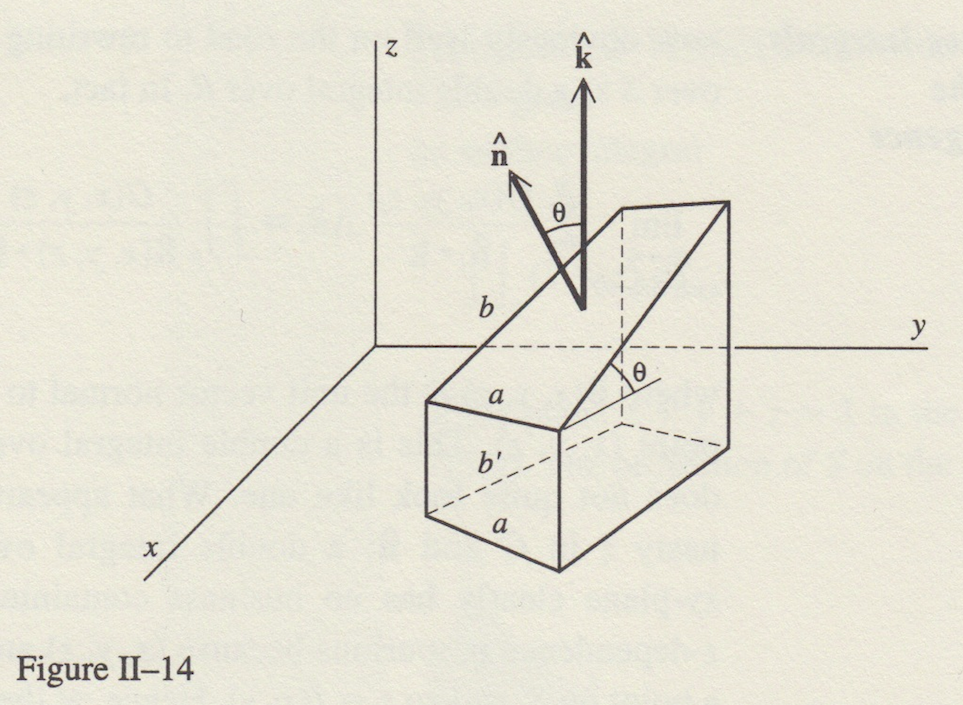
\includegraphics [scale=0.3] {tilt.png} \end{center}

\[ \cos \theta = \hat{\mathbf{n}} \cdot \hat{\mathbf{k}} \]

 the side that will shrink is the hypotenuse of a triangle, where the new length divided by that hypotenuse is just $\cos \theta$.  That is

\[ b' = b \cos \theta = b \ \hat{\mathbf{n}} \cdot \hat{\mathbf{k}} \]

Since the area is the product of adjacent sides, the shrinkage factor is the same as above, that is

\[ dR = dS \ \cos \theta = dS \ \hat{\mathbf{n}} \cdot \hat{\mathbf{k}} \]

and therefore

\[ \iint_S G(x,y,z)  \ dS =  \iint_R G(x,y,z)  \ \frac{dR}{\hat{\mathbf{n}} \cdot \hat{\mathbf{k}}} \]
\[ = \iint_R G(x,y,z)  \ \frac{1}{\hat{\mathbf{n}} \cdot \hat{\mathbf{k}}} \ dx \ dy \]

Notice that we have $G(x,y,z)$ but only $dx \ dy$.  However, this is no problem once we recall that $z$ is a function $f(x,y)$ (according to the definition of our surface).  So we can rewrite this as

\[ \iint_R G(x,y,f(x,y))  \ \frac{1}{\hat{\mathbf{n}} [x,y,f(x,y)] \cdot \hat{\mathbf{k}}} \ dx \ dy \]

Furthermore, we showed above that

\[  \hat{\mathbf{n}} = \frac{1}{\sqrt{f_x^2  + f_y^2 + 1}} \ < \ -f_x, - f_y , 1  \ > \]
\[  \hat{\mathbf{n}} \cdot \hat{\mathbf{k}} = \frac{1}{\sqrt{f_x^2  + f_y^2 + 1}} \ (1)   \]

So again we rewrite the surface integral as

\[ \iint_R G(x,y,f(x,y))  \ \sqrt{f_x^2  + f_y^2 + 1}  \ dx \ dy \]

\noindent\rule{15cm}{0.4pt}

\subsection*{examples}

Some examples will make this all more concrete.

Suppose we have as our surface the plane that cuts through $(1,0,0)$, $(0,1,0)$, and $(0,0,1)$.  We're given the equation of the plane:

\[ x + y + z = 1 \]

which we can guess in this special case, but if necessary we could find two vectors in the plane (say $<1,-1,0>$ and $<1,0,-1>$, take their cross product to get the normal vector $<1,1,1>$, and then plug in a point to solve $ax + by + cz = d$ and get $d=1$.  We are also given that $G(x,y,z) = x + z$.  So, using the equations from before, the surface integral is

\[ \iint_S G(x,y,f(x,y)) \ dS \]
\[ \iint_R G(x,y,f(x,y))  \ \sqrt{f_x^2  + f_y^2 + 1}  \ dx \ dy \]

Rearrange the plane equation to give $z = 1 - x - y$.  So, $f_x = -1$ and $f_y = -1$.  Similarly $G(x,y,z) = x + z = x + 1 - x - y = 1 - y$, so we obtain

\[ \iint_R (1-y)  \ \sqrt{3}  \ dx \ dy \]
\[ = \sqrt{3} \ [ \ \iint_R 1  \ dx \ dy - \ \iint_R y  \ dx \ dy \ ] \ \]

Like most double integrals, the tricky part is to set up the bounds.  Here our region $R$ is bounded on the top by a line going through $(0,1)$ and $(1,0)$.  The equation of this line is $x + y = 1;  y = 1 - x$.  So if we integrate $y$ from $0 \rightarrow 1$, we integrate $x$ from $0 \rightarrow 1-y$.

\[ = \sqrt{3} \ [ \int_0^1 \int_0^{1-y} 1  \ dx \ dy - \ \int_0^1 \int_0^{1-y} y  \ dx \ dy \ ] \ \]
\[ = \sqrt{3} \ [ \int_0^1 (1-y) \ dy - \ \int_0^1 y-y^2 \ dy \ ] \ \]
\[ = \sqrt{3} \ [ (y - \frac{1}{2}y^2) \ \bigg |_0^1 - (\frac{1}{2}y^2 - \frac{1}{3}y^3) \ \bigg |_0^1 \ ] \ \]
\[ = \sqrt{3} \ ( \ 1 - \frac{1}{2} - \frac{1}{2} + \frac{1}{3} ) = \frac{1}{\sqrt{3}} \]

The second problem involves the unit sphere.  Here the equation of our surface is
\[ x^2 + y^2 + z^2 = 1 \]
and we're just looking at the octant which has $x,y,z > 0$.  

The function we want to integrate is
\[ \iint_S z^2 \ dS \]
Rearranging the first equation we have:
\[ z = \sqrt{1 - x^2 - y^2} \]
Recall that
\[ f_x = -\frac{x}{z} \]
\[ f_y = -\frac{y}{z} \]
so

\[ \iint_R G(x,y,f(x,y))  \ \sqrt{f_x^2  + f_y^2 + 1}  \ dx \ dy \]
\[ = \iint_R z^2  \ \sqrt{(\frac{x}{z})^2  + (\frac{y}{z})^2 + 1}  \ dx \ dy \]
\[ = \iint_R z^2  \frac{1}{z} \ \sqrt{x^2  + y^2 + z^2 }  \ dx \ dy \]
\[ = \iint_R z \ dx \ dy \]
\[ = \iint_R \sqrt{1 - x^2 - y^2} \ dx \ dy \]

Switch to polar coordinates
\[ x = r \cos \theta \]
\[ y = r \sin \theta \]
\[ z = \sqrt{1 - x^2 - y^2} \]
\[ = \sqrt{1 - r^2\cos^2 \theta - r^2\sin^2 \theta } \]
\[ = \sqrt{1 - r^2} \]

To convert to $dr$ and $d\theta$ we need the Jacobian
\[ dx \ dy = r \ dr \ d\theta \]
So we have

\[ = \iint_R \sqrt{1 - r^2} \ r \ dr \ d\theta \]
\[ = \int_0^{pi/2}  \int_{r=0}^{r=1} \sqrt{1 - r^2} \ r \ dr \ d\theta \]
\[ = \int_0^{pi/2} [-\frac{1}{3}(1-r^2)^{3/2}] \ \bigg |_0^1 ] \ d \theta \]
\[ =  \int_0^{pi/2} \frac{1}{3} \ d \theta = \frac{\pi}{6} \]

\noindent\rule{15cm}{0.4pt}

\subsection*{vector field}
To finish up, let's go back to

\[ \iint_S \mathbf{F} \cdot \hat{\mathbf{n}} \ dS \]

in $x,y$-coordinates, this is

\[ \hat{\mathbf{n}} \ dS = < -f_x,-f_y,1>  \ dx \ dy \]

How do we get this?  Above we derived an expression for the surface element $dS$

\[ dS = \ \sqrt{f_x^2 + f_y^2 + a} \ dx \ dy \]

so in $R$ the integral becomes

\[ \iint_R \mathbf{F} \cdot \hat{\mathbf{n}} \ \sqrt{1 + f_x^2 + f_y^2} \ dx \ dy \]

Recall from earlier that

\[  \hat{\mathbf{n}} = \frac{\mathbf{u} \times \mathbf{v}}{| \mathbf{u} \times \mathbf{v} |} = \frac{1}{\sqrt{f_x^2  + f_y^2 + 1}} \ < -f_x, - f_y , 1 > \]

The square root cancels, leaving us with

\[ \iint_R \mathbf{F} \cdot \ < -f_x,-f_y,1>  \ dx \ dy \]

\subsection*{example 1}

Suppose that
\[ \mathbf{F} = z \hat{\mathbf{i}} - y \hat{\mathbf{j}} + x  \hat{\mathbf{k}} \]
\[ \mathbf{F} = \ <z,-y,x> \]
and $S$ is the part of the plane $x + 2y + 2z = 2$ in the positive octant, crossing through the points $(2,0,0),(0,1,0)$ and $(0,0,1)$.

Rearrange the equation of the surface
\[ f(x,y) = z = 1 - \frac{x}{2} - y \]
\[ f_x = -\frac{1}{2} \]
\[ f_y = -1 \]

We want to compute
\[ \iint_R \mathbf{F} \cdot \ < -f_x,-f_y,1>  \ dx \ dy \]

Plugging in
\[ \mathbf{F} \cdot \ < -f_x,-f_y,1> \]
\[ = \ <z,-y,x> \ \cdot \ < \frac{1}{2},1,1> \]
\[ = \frac{1}{2}(1 - \frac{x}{2} - y) - y + x \]
\[ = \frac{1}{2} + \frac{3}{4}x - \frac{3}{2}y \]
So the integral is
\[ =  \iint_R \ \frac{1}{2} + \frac{3}{4}x - \frac{3}{2}y  \ dx \ dy \]

If we integrate with respect to $dy$ first, using $y = 0 \rightarrow y = -x/2 + 1$, the inner integral is
\[ = \frac{1}{2} y + \frac{3}{4}xy - \frac{3}{4} y^2 \  \bigg |_{y=0}^{y = -x/2 + 1} \]
\[ = \frac{1}{2}(-\frac{x}{2} + 1) + \frac{3}{4}x(-\frac{x}{2} + 1) -  \frac{3}{4}(-\frac{x}{2} + 1)^2 \]
Now
\[ (-\frac{x}{2} + 1)^2 = \frac{x}{4} -x + 1\]
 so we have
 \[ = \frac{1}{2}(-\frac{x}{2} + 1) + \frac{3}{4}x(-\frac{x}{2} + 1) -  \frac{3}{4}(\frac{x}{4} -x + 1) \]
\[ = -\frac{x}{4} + \frac{1}{2} - \frac{3}{8}x^2 + \frac{3}{4}x - \frac{3}{16}x + \frac{3}{4}x - \frac{3}{4} \]
\[ = - \frac{1}{4} -\frac{x}{4} - \frac{3}{8}x^2 + \frac{3}{4}x - \frac{3}{16}x + \frac{3}{4}x \]
\[ = - \frac{1}{4} +\frac{5}{4}x  - \frac{3}{16}x - \frac{3}{8}x^2  \]
\[ = - \frac{1}{4} + \frac{17}{16}x  - \frac{3}{8}x^2 \  \]
and then the inner integral is
\[ = - \frac{1}{4}x + \frac{17}{32}x^2  - \frac{1}{8}x^3 \  \bigg |_0^1 = \frac{5}{32}  \]
The answer given is $1/2$ so I suppose there is a mistake somewhere..
\subsection*{example 2}

Take the surface of the unit sphere ($z = \sqrt{1-x^2-y^2}$ in the positive octant.  The region $R$ in the $xy$-plane is the unit circle in that quadrant.

We find $f_x = -x/z$ and $f_y = -y/z$ as usual and 
\[ \mathbf{F} = xz \hat{\mathbf{i}} + z^2 \hat{\mathbf{k}} \]
\[ \mathbf{F} = \ <xz,0,z^2> \]
So 
\[ \mathbf{F} \cdot \ < -f_x,-f_y,1> \]
\[ = \ <xz,0,z^2> \ \cdot \ < \frac{x}{z},\frac{y}{z},1> \]
\[ = x^2 + z^2 \]
\[ = x^2 + 1 - x^2 - y^2 \]
We want compute
\[ = \iint_R 1 -y^2 \ dx \ dy \]

The first part of this integral is just the area of the quarter circle of radius $1$, equal to $\pi/4$.
For the second term, we want to integrate over the same region, which suggests the use of polar coordinates 
\[ x = r \cos \theta \]
\[ y = r \sin \theta \]
\[ \iint_R y^2 \ dx \ dy \]
\[ = \int_0^{\pi/2} \int_0^1 r^2 \sin^2 \theta \ r \ dr \ d \theta \]

If we do $r^3 dr$ first we get a factor of $1/4$ so we have 
\[ \frac{1}{4} \int_0^{\pi/2} \sin^2 \theta \ d \theta \]
\[ = \frac{1}{4} \frac{1}{2}(\theta - \frac{1}{2}\sin 2 \theta) \  \bigg |_0^{\pi/2}  \]
\[ = \frac{1}{8} (\frac{\pi}{2}) \]
Combining with $\pi/4$ (and remembering the minus sign)
\[ = \frac{\pi}{4} - \frac{\pi}{16} = \frac{3}{16} \pi \]

\end{document}  